\section{Đề số 32}

\begin{bt} 
	\hfill
	\begin{enumerate}[a.]
		\item Tính giá trị của biểu thức $\mathrm{A}=\left(\frac{-4}{7}+\frac{2}{5}\right): \frac{2}{3}+\left(\frac{-3}{7}+\frac{3}{5}\right): \frac{2}{3}$
		\item Tính giá trị của biểu thức $\mathrm{B}=2 \mathrm{x}^2-3 \mathrm{x}+1$ với $|x|=\frac{1}{2}$.
		\item Tìm 3 số $x, y, z$ biết rằng: $\frac{x}{3}=\frac{y}{7} ; \frac{y}{2}=\frac{z}{5}$ và $x+y+z=-110$.
	\end{enumerate}
	\loigiai{
		\begin{enumerate}
			\item $A=\left(\frac{-4}{7}+\frac{2}{5}\right): \frac{2}{3}+\left(\frac{-3}{7}+\frac{3}{5}\right): \frac{2}{3} \\[5px]
			=\left(\frac{-4}{7}+\frac{2}{5}+\frac{-3}{7}+\frac{3}{5}\right): \frac{2}{3} \\[5px]
			=\left[\left(\frac{-4}{7}+\frac{-3}{7}\right)+\left(\frac{2}{5}+\frac{3}{5}\right)\right]: \frac{2}{3}=0: \frac{2}{3}=0$\\[5px]
			Vậy : $A=0$
			\item Vì $|x|=\frac{1}{2}$ nên $\mathrm{x}=\frac{1}{2}$ hoặc $\mathrm{x}=-\frac{1}{2}$\\[5px]
			Với $\quad x=\frac{1}{2}$ thì: $A=2 \cdot\left(\frac{1}{2}\right)^2-3 \cdot \frac{1}{2}+1=0$\\[5px]
			Với $x=-\frac{1}{2}$ thì: $A=2 .\left(-\frac{1}{2}\right)^2-3 .\left(-\frac{1}{2}\right)+1=3$\\[5px]
			Vậy : $\mathrm{A}=0$ với $\mathrm{x}=\frac{1}{2}$ và $\mathrm{A}=3$ với $\mathrm{x}=-\frac{1}{2}$
			\item Từ $\frac{\mathrm{x}}{3}=\frac{\mathrm{y}}{7} \Rightarrow \frac{\mathrm{x}}{6}=\frac{\mathrm{y}}{14} ; \frac{\mathrm{y}}{2}=\frac{\mathrm{z}}{5} \Rightarrow \frac{\mathrm{y}}{14}=\frac{\mathrm{z}}{35}$. Suy ra $\frac{\mathrm{x}}{6}=\frac{\mathrm{y}}{14}=\frac{\mathrm{z}}{35}$\\[5px][5px]
			Áp dụng tính chất của dãy tỉ số bằng nhau, ta có:\\[5px]
			$\frac{x}{6}=\frac{y}{14}=\frac{z}{35}=\frac{x+y+z}{6+14+35}=\frac{-110}{55}=-2 \\[5px]
			\text {Suy ra } x=-2.6=-12 ; \quad y=-2.14=-28 ; z=-2.35=-70 . \\[5px]
			\text {Vậy: } x=-12 ; \quad y=-28 ; z=-70 .$
		\end{enumerate}
	} 
\end{bt}

\begin{bt}
	\hfill
	\begin{enumerate}[a.]
		\item Tìm tập hợp các số nguyên $x$, biết rằng:
		$$
		4 \frac{5}{9}: 2 \frac{5}{18}-7<x<\left(3 \frac{1}{5}: 3,2+4,5.1 \frac{31}{45}\right):\left(-21 \frac{1}{2}\right)
		$$
		\item Cho $\frac{a}{c}=\frac{c}{b}$. Chứng minh rằng: $\frac{a^2+c^2}{b^2+c^2}=\frac{a}{b}$
		\item Tính giá trị của biểu thức: $C=2 x^5-5 y^3+2015$ tại $x, y$ thỏa mãn:
		$$	|x-1|+(y+2)^{20}=0 $$
	\end{enumerate}
	\loigiai{
		\begin{enumerate}
			\item Ta có: $4 \frac{5}{9}: 2 \frac{5}{18}-7=\frac{41}{9} \cdot \frac{18}{41}-7=2-7=-5$\\[5px]
			Lại có: $\left(3 \frac{1}{5}: 3,2+4,5 \cdot 1 \frac{31}{45}\right):\left(-21 \frac{1}{2}\right)=\left(\frac{16}{5} \cdot \frac{5}{16}+\frac{9}{2} \cdot \frac{76}{45}\right):\left(-\frac{43}{2}\right)=\left(1+\frac{38}{5}\right) \cdot \frac{-2}{43}\\[5px][5px]
			=\frac{43}{5} \cdot \frac{-2}{43}=\frac{-2}{5}$\\[5px]
			Do đó: $-5<x<\frac{-2}{5}$ mà $x \in Z$ nên $x \in\{-4 ;-3 ;-2 ;-1\}$
			\item Do $|x-1| \geq 0$; $(\mathrm{y}+2)^{20} \geq 0 \Rightarrow|x-1|+(\mathrm{y}+2)^{20} \geq 0$ vói mọi $\mathrm{x}, \mathrm{y}$.\\[5px]
			Kết hợp $|x-1|+(\mathrm{y}+2)^{20}=0$ suy ra $|x-1|=0$ và $(\mathrm{y}+2)^{20}=0$ $\Leftrightarrow x=1 ; y=-2$\\[5px][5px]
			Giá trị của biểu thức : $C=2 x^5-5 y^3+2015$ tại $x=1 ; y=-2$ là:\\[5px][5px]
			$C=2 \cdot 1^5-5 \cdot(-2)^3+2015=2+40+2015=2057$\\[5px][5px]Vậy $C=2057$
		\end{enumerate}
	} 
\end{bt}

\begin{bt}
	\hfill 
	\begin{enumerate}[a.]
		\item Tìm số tự nhiên có ba chữ số, biết rằng số đó là bội của 18 và các chữ số của nó tỉ lệ theo 1: 2: 3.
		\item Tìm tất cả các số tự nhiên $a, b$ sao cho : $2^{\mathrm{a}}+37=|b-45|+\mathrm{b}-45$.
	\end{enumerate}
	\loigiai{
		\begin{enumerate}
			\item Gọi a, b, c là các chữ số của số có ba chữ số cân tìm. Không mất tính tổng quát, giả sử a $\leq \mathrm{b} \leq \mathrm{c} \leq 9$\\[5px]
			Ta có $1 \leq \mathrm{a}+\mathrm{b}+\mathrm{c} \leq 27$.\\[5px]
			Mặt khác số cần tìm là bội của 18 nên là bội của 9 , do đó $a+b+c=9$ hoặc $a+b+c=18$ hoặc $a+b+c=27$.\\[5px]
			Theo đề bài ta có: $\frac{a}{1}=\frac{b}{2}=\frac{c}{3}=\frac{a+b+c}{6}$;\\[5px]
			Như vậy $a+b+c$ chia hết cho 6 , nên $a+b+c=18$.\\[5px]
			Từ đó suy ra $\mathrm{a}=3, \mathrm{~b}=6, \mathrm{c}=9$.\\[5px]
			Do số phải tìm là bội của 18 nên chữ số hàng đơn vị chẵn,\\[5px][5px]
			vì vậy hai số cân tìm là: 396; 936.
			\item Từ $\frac{a}{c}=\frac{c}{b}$ suy ra $c^2=a \cdot b$\\[5px]
			khi đó $\frac{a^2+c^2}{b^2+c^2}=\frac{a^2+a \cdot b}{b^2+a \cdot b}=\frac{a(a+b)}{b(a+b)}=\frac{a}{b}$
			\item Nhận xét: Với $x \geq 0$ thì $|x|+x=2 x$\\[5px]
			Với $x<0$ thì $|x|+x=0$. Do đó $|x|+x$ luôn là số chẵn với $\forall x \in Z$.\\[5px]
			Áp dụng nhận xét trên thì $|\mathrm{b}-45|+\mathrm{b}-45$ là số chẵn với $\mathrm{b} \in \mathrm{Z}$.\\[5px]
			Suy ra $2^a+37$ là số chẵn $\Rightarrow 2^a$ lẻ $\Leftrightarrow a=0$.\\[5px]
			Khi đó $|\mathrm{b}-45|+\mathrm{b}-45=38$\\[5px]
			+ Nếu $b<45$, ta có $-(b-45)+b-45=38 \Leftrightarrow 0=38$ (loại)\\[5px]
			+ Nếu $b \geq 45$, ta có $2(b-45)=38 \Leftrightarrow b-45=19 \Leftrightarrow \mathrm{b}=64(\mathrm{TM})$\\[5px]
			vậy $(a ; b)=(0 ; 64)$
		\end{enumerate}
	} 
\end{bt}

\begin{bt}
	Cho tam giác $\mathrm{ABC}$ có ba góc nhọn $(\mathrm{AB}<\mathrm{AC})$. Vẽ về phía ngoài tam giác $A B C$ các tam giác đều $A B D$ và $A C E$. Gọi $I$ là giao của $C D$ và $B E, K$ là giao của $A B$ và $D C$.
	\begin{enumerate}[a.]
		\item Chứng minh rằng: $\triangle \mathrm{ADC}=\triangle \mathrm{ABE}$.
		\item Chứng minh rằng: góc $\mathrm{DIB}=60^{\circ}$.
		\item Gọi $\mathrm{M}$ và $\mathrm{N}$ lân lượt là trung điểm của $\mathrm{CD}$ và $\mathrm{BE}$. Chứng minh rằng $\triangle \mathrm{AMN}$ đều.
		\item Chứng minh rằng IA là phân giác của góc DIE.
	\end{enumerate}
	\loigiai{
		$$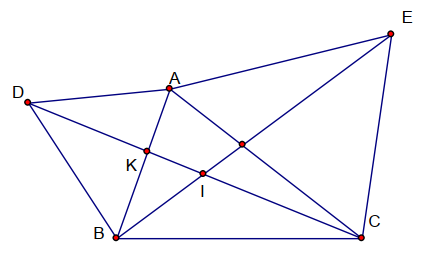
\includegraphics[width=0.55\textwidth]{32-4-lg.png}$$
		\begin{enumerate}
			\item Ta có: $\mathrm{AD}=\mathrm{AB} ; \mathrm{DAC}=\mathrm{BAE}$ và $\mathrm{AC}=\mathrm{AE}$\\[5px]
			Suy ra $\triangle \mathrm{ADC}=\triangle \mathrm{ABE}$ (c.g.c)
			\item Từ $\triangle \mathrm{ADC}=\triangle \mathrm{ABE}$ (câu a) $\Rightarrow \mathrm{ABE}=\mathrm{ADC}$,\\[5px]
			mà $\mathrm{BKI}=\mathrm{AKD}$ (đối đỉnh).\\[5px]
			Khi đó xét $\triangle \mathrm{BIK}$ và $\triangle \mathrm{DAK}$ suy ra $\mathrm{BIK}=\mathrm{DAK}=60^{\circ}(\mathrm{đpcm})$
			\item $$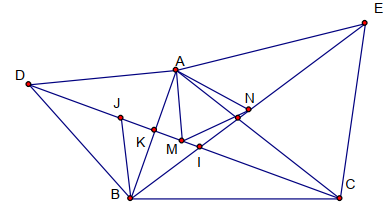
\includegraphics[width=0.55\textwidth]{32-4.2-lg.png}$$
			$\text {Từ } \triangle \mathrm{ADC}=\triangle \mathrm{ABE} \text { (câu a) } \Rightarrow \mathrm{CM}=\mathrm{EN} \text { và } \mathrm{ACM}=\mathrm{AEN} \\[5px]
			\Rightarrow \triangle \mathrm{ACM}=\triangle \mathrm{AEN} \text { (c.g.c) } \Rightarrow \mathrm{AM}=\mathrm{AN} \text { và } \mathrm{CAM}=\mathrm{EAN} \\[5px]
			\mathrm{MAN}=\mathrm{CAE}=60^{\circ} \text {. Do đó } \triangle \mathrm{AMN} \text { đều. }$
			\item Trên tia ID lấy điểm $\mathrm{J}$ sao cho $\mathrm{IJ}=\mathrm{IB} \Rightarrow \Delta \mathrm{BIJ}$ đều $\Rightarrow \mathrm{BJ}=\mathrm{BI}$ và $\mathrm{JBI}=\mathrm{DBA}=60^{\circ}$\\[5px][5px]
			suy ra $\mathrm{IBA}=\mathrm{JBD}$, kết hợp $\mathrm{BA}=\mathrm{BD}$\\[5px]
			$\Rightarrow \Delta \mathrm{IBA}=\Delta \mathrm{JBD} \text { (c.g.c) } \Rightarrow \mathrm{AIB}=\mathrm{DJB}=120^{\circ} \text { mà } \mathrm{BID}=60^{\circ}$\\[5px]
			$\Rightarrow \mathrm{DIA}=60^{\circ}$. Từ đó suy ra IA là phân giác của góc $\mathrm{DIE}$
		\end{enumerate}
	}
\end{bt}

\begin{bt}
	Cho 20 số nguyên khác $0: a_1, a_2, a_3, \ldots, a_{20} $ có các tính chất sau: 
	\begin{itemize}[*]
		\item $a_1$ là số dương.
		\item Tổng của ba số viết liền nhau bất kì là một số dương.
		\item Tổng của 20 số đó là số âm.
	\end{itemize}
	Chứng minh rằng : $a_{1} . a_{14}+ a_{14} . a_{12}<a_1 \cdot a_{12}$.
	\loigiai{
		Ta có:\\[5px]
		$a_1+\left(a_2+a_3+a_4\right)+\ldots+\left(a_{11}+a_{12}+a_{13}\right)+a_{14}+\left(a_{15}+a_{16}+a_{17}\right)+\left(a_{18}+a_{19}+a_{20}\right)<0 ; a_1>0 ; \\[5px]
		a_2+a_3+a_4>0 ; \ldots ; a_{11}+a_{12}+a_{13}>0 ; a_{15}+a_{16}+a_{17}>0 ; a_{18}+a_{19}+a_{20}>0 \Rightarrow a_{14}<0$\\[5px]
		Cũng như vậy :\\[5px]
		$\left(a_1+a_2+a_3\right)+\ldots+\left(a_{10}+a_{11}+a_{12}\right)+\left(a_{13}+a_{14}\right)+\left(a_{15}+a_{16}+a_{17}\right)+\left(a_{18}+a_{19}+a_{20}\right)$ $<0=>\mathrm{a}_{13}+\mathrm{a}_{14}<0$\\[5px]
		Mặt khác, $\mathrm{a}_{12}+\mathrm{a}_{13}+\mathrm{a}_{14}>0 \Rightarrow \mathrm{a}_{12}>0$.\\[5px]
		Từ các điều kiện $a_1>0 ; a_{12}>0 ; a_{14}<0 \\[5px]
		\Rightarrow a_1 \cdot a_{14}+a_{14} a_{12}<a_1 \cdot a_{12}$ (đpcm).
	}
\end{bt}
